%% FEUP THESIS STYLE for LaTeX2e
%% how to use feupteses (English version)
%%
%% FEUP, JCL & JCF, 31 July 2012
%%
%% PLEASE send improvements to jlopes at fe.up.pt and to jcf at fe.up.pt
%%

%%========================================
%% Commands: pdflatex tese
%%           bibtex tese
%%           makeindex tese (only if creating an index)
%%           pdflatex tese
%% Alternative:
%%          latexmk -pdf tese.tex
%%========================================

\documentclass[11pt,a4paper,twoside,openright]{report}

%% For iso-8859-1 (latin1), comment next line and uncomment the second line
\usepackage[utf8]{inputenc}
%\usepackage[latin1]{inputenc}

%% English version

%% MIEIC options
\usepackage[mieic]{feupteses}
%\usepackage[mieic,juri]{feupteses}
%\usepackage[mieic,final]{feupteses}
%\usepackage[mieic,final,onpaper]{feupteses}

% For gantt timeline diagrams
\usepackage{pgfgantt}

% For tables
\usepackage{multirow}

% For superscript
\usepackage{fixltx2e}

% For glossary
\usepackage[acronym]{glossaries}

\usepackage{natbib}

%% Additional options for feupteses.sty: 
%% - onpaper: links are not shown (for paper versions)
%% - backrefs: include back references from bibliography to citation place

%% Uncomment the next lines if side by side graphics used
%\usepackage[lofdepth,lotdepth]{subfig}
%\usepackage{graphicx}
%\usepackage{float}

%% Include color package
\usepackage{color}
\definecolor{cloudwhite}{cmyk}{0,0,0,0.025}
\definecolor{Apricot}{HTML}{FBB982}
\newcommand{\apiname}{SAJaS} 
\newcommand{\apilongname}{Simple API for JADE-based Simulations}

%%% For charts%%
\usepackage{tikz}



%% Include source-code listings package
\usepackage{listings}
\lstset{ %
 language=Java,                        % choose the language of the code
 basicstyle=\footnotesize\ttfamily,
 keywordstyle=\bfseries,
 numbers=left,                      % where to put the line-numbers
 numberstyle=\scriptsize\texttt,    % the size of the fonts that are used for the line-numbers
 stepnumber=1,                      % the step between two line-numbers. If it's 1 each line will be numbered
 numbersep=8pt,                     % how far the line-numbers are from the code
 frame=tb,
 float=htb,
 aboveskip=8mm,
 belowskip=4mm,
 backgroundcolor=\color{cloudwhite},
 showspaces=false,                  % show spaces adding particular underscores
 showstringspaces=false,            % underline spaces within strings
 showtabs=false,                    % show tabs within strings adding particular underscores
 tabsize=2,                     % sets default tabsize to 2 spaces
 captionpos=b,                      % sets the caption-position to bottom
 breaklines=true,                   % sets automatic line breaking
 breakatwhitespace=false,           % sets if automatic breaks should only happen at whitespace
 escapeinside={\%*}{*)},            % if you want to add a comment within your code
 morekeywords={*,var,template,new}  % if you want to add more keywords to the set
}
%% For code block %%
\lstset{basicstyle=\footnotesize\ttfamily,breaklines=true}
\lstset{framextopmargin=0pt,frame=lrbt,rulecolor=\color{Gray}}
%%%

%% Uncomment to create an index (at the end of the document)
%\makeindex

%% Path to the figures directory
%% TIP: use folder ``figures'' to keep all your figures
\graphicspath{{figures/}}

%\makeglossaries

%%----------------------------------------
%% TIP: if you want to define more macros, use an external file to keep them
%some macro definitions

% format
\newcommand{\class}[1]{{\normalfont\slshape #1\/}}

% entities
\newcommand{\Feup}{Faculdade de Engenharia da Universidade do Porto}

\newcommand{\svg}{\class{SVG}}
\newcommand{\scada}{\class{SCADA}}
\newcommand{\scadadms}{\class{SCADA/DMS}}

%%----------------------------------------

%%========================================
%% Start of document
%%========================================
\begin{document}

%%----------------------------------------
%% Information about the work
%%----------------------------------------
\title{From simulation to development in MAS: Repast-JADE automatic code generation for interaction protocols}
\author{João Pedro Camacho Lopes}

%% Uncomment next line for date of submission
%\thesisdate{July 31, 2008}

%%Uncomment next line for copyright text if used
%\copyrightnotice{Name of the Author, 2008}

\supervisor{Supervisor}{Henrique Lopes Cardoso}

%% Uncomment next line if necessary
%\supervisor{Second Supervisor}{Name of the Supervisor}

%% Uncomment committee stuff in the final version if used
%\committeetext{Approved in oral examination by the committee:}
%\committeemember{Chair}{Doctor Name of the President}
%\committeemember{External Examiner}{Doctor Name of the Examiner}
%\committeemember{Supervisor}{Doctor Name of the Supervisor}
%\signature

%% Specify cover logo (in folder ``figures'')
\logo{uporto-feup.pdf}

%% Uncomment next line for additional text  below the author's name (front page)
\additionalfronttext{}

%%----------------------------------------
%% Preliminary materials
%%----------------------------------------

% remove unnecssary \include{} commands
\begin{Prolog}
  %!TEX root = thesis.tex
\chapter*{Abstract}

%Multi-agent systems (MAS) present an interesting approach to the efficient development of modular systems. MAS are composed by autonomous computational units called agents that are programmed to \emph{compete} or \emph{work together}, for instance in order to solve computational problems, engage in automatic negotiation or play computer games. Frameworks exist that aid the development of this class of systems and they range from mostly general-purpose frameworks to domain-specific in an array of different domains.
%
%Multi-agent-based simulations (MABS) are sometimes used on the course of development of a full-featured MAS - for instance, for testing purposes. However, most platforms for MAS development are not well suited for MABS development \cite{mengistu2008scalability}.
%
%JADE \cite{bellifemine2003jade}, a very popular MAS development framework allows the creation of seamless distributed agent systems and complies with FIPA standards for agent interaction. Unfortunately, its multi-threaded architecture falls short in delivering the necessary performance to run a local simulation with a large number of agents. Repast \cite{collier2003repast} is an agent-based simulation toolkit that allows creating simulations using rich GUI elements and real time agent statistics. Unlike JADE, though, Repast lacks much of the infrastructure for agent creation and interaction.
%
%Some authors \cite{garcia2011misia,gormer2011jrep}, as reviewed in this report, proposed an integration of JADE and Repast by means of a middleware, essentially representing the agent in both and taking advantage of the features provided by the frameworks.
%
%In this thesis, a code generation tool is proposed, capable of not only generating a Repast simulation from an existing JADE MAS, but also of creating a full featured JADE application from a Repast-based simulation. An implementation of FIPA's interaction protocols will be proposed for Repast as a means to deliver the mentioned conversion tool. The most immediate advantage over the previous approaches is that existing systems can make use of this tool to create appropriate simulations where agent interaction can be more easily analyzed. Furthermore, proficient programmers in one framework can quickly get started in the development for the complementary framework.


\chapter*{Resumo}
%
%Os sistemas multi-agente (SMA) exprimem uma abordagem interessante no desenvolvimento de sistemas modulares e eficientes. Os MAS são compostos por elementos computacionais autónomos - chamados agentes - que são programados para \emph{competir} ou \emph{colaborar} de modo a, por exemplo, resolver problemas computacionais, iniciar negociação automática ou participar em jogos de computador. Existem ferramentas de software que facilitam o desenvolvimento desta classe de sistemas que podem variar entre ferramentas de âmbito geral até ferramentas focadas num domínio específico.
%
%As simulações baseadas em agente (SBA) são frequentemente utilizadas durante o desenvolvimento de MAS completos - por exemplo, afim de testar o sistema. No entanto, a maior parte das plataformas para desenvolvimento de SMA não são apropriadas para a criação de SBA \cite{mengistu2008scalability}.
%
%O JADE \cite{bellifemine2003jade} é um exemplo de uma plataforma de desenvolvimento de SMA que permite a criação de sistemas distribuídos de agentes de forma simplificada cumprindo, ainda, os standards da FIPA (\emph{Foundation for Intelligent Physical Agents}) sobre protocolos de interação entre agentes. No entanto, a sua arquitetura em \emph{multi-thread} não garante a performance necessária para a execução de simulações com um elevado número de agentes. O Repast \cite{collier2003repast} é uma plataforma de criação de simulações baseadas em agentes que permite criar simulações ricas em interfaces gráficas para visualização de dados históricos e em tempo real sobre os agentes. Ao contrário do JADE, o Repast não dispõe de uma infraestrutura para criação de agentes e interação entre eles.
%
%Alguns autores estudados neste relatório \cite{garcia2011misia,gormer2011jrep} propõem uma integração entre o JADE e o Repast por meio de uma camada de software intermédio, fazendo representar cada agente duplamente - uma vez em cada plataforma, essencialmente tirando partido das capacidades de ambas as plataformas em simultâneo.
%
%Para esta dissertação é proposta uma ferramenta de geração automática de código capaz não só de gerar uma simulação baseada em Repast a partir de um SMA baseado em JADE, mas também de criar um SMA em JADE partindo de uma simulação baseada em Repast. Será também criada uma proposta de implementação, para a plataforma Repast, dos standards da de interação entre agentes da FIPA, tornando possível a conversão de código entre as duas plataformas. A vantagem mais imediata sobre a proposta anterior é que SMA já existentes podem tirar partido da ferramenta proposta para rapidamente criar uma simulação com funcionamento equivalente e ter acesso a ferramentas de visualização e estatísticas do sobre o comportamento dos agentes. Adicionalmente, programadores proficientes numa das plataformas pode iniciar rapidamente o desenvolvimento da plataforma complementar. % the abstract
  % \chapter*{Acknowledgements}

Aliquam id dui. Nulla facilisi. Nullam ligula nunc, viverra a, iaculis
at, faucibus quis, sapien. Cum sociis natoque penatibus et magnis dis
parturient montes, nascetur ridiculus mus. Curabitur magna ligula,
ornare luctus, aliquam non, aliquet at, tortor. Donec iaculis nulla
sed eros. Sed felis. Nam lobortis libero. Pellentesque
odio. Suspendisse potenti. Morbi imperdiet rhoncus magna. Morbi
vestibulum interdum turpis. Pellentesque varius. Morbi nulla urna,
euismod in, molestie ac, placerat in, orci. 

Ut convallis. Suspendisse luctus pharetra sem. Sed sit amet mi in diam
luctus suscipit. Nulla facilisi. Integer commodo, turpis et semper
auctor, nisl ligula vestibulum erat, sed tempor lacus nibh at
turpis. Quisque vestibulum pulvinar justo. Class aptent taciti
sociosqu ad litora torquent per conubia nostra, per inceptos
himenaeos. Nam sed tellus vel tortor hendrerit pulvinar. Phasellus
eleifend, augue at mattis tincidunt, lorem lorem sodales arcu, id
volutpat risus est id neque. Phasellus egestas ante. Nam porttitor
justo sit amet urna. Suspendisse ligula nunc, mollis ac, elementum
non, venenatis ut, mauris. Mauris augue risus, tempus scelerisque,
rutrum quis, hendrerit at, nunc. Nulla posuere porta orci. Nulla dui. 

Fusce gravida placerat sem. Aenean ipsum diam, pharetra vitae, ornare
et, semper sit amet, nibh. Nam id tellus. Etiam ultrices. Praesent
gravida. Aliquam nec sapien. Morbi sagittis vulputate dolor. Donec
sapien lorem, laoreet egestas, pellentesque euismod, porta at,
sapien. Integer vitae lacus id dui convallis blandit. Mauris non
sem. Integer in velit eget lorem scelerisque vehicula. Etiam tincidunt
turpis ac nunc. Pellentesque a justo. Mauris faucibus quam id
eros. Cras pharetra. Fusce rutrum vulputate lorem. Cras pretium magna
in nisl. Integer ornare dui non pede. 

\vspace{10mm}
\flushleft{The Name of the Author}
  % the acknowledgments
  % \cleardoublepage
\thispagestyle{plain}

\vspace*{8cm}

\begin{flushright}
   \textsl{``You should be glad that bridge fell down. \\
           I was planning to build thirteen more to that same design''} \\
\vspace*{1.5cm}
           Isambard Kingdom Brunel
\end{flushright}
       % initial quotation if desired
  \cleardoublepage
  \pdfbookmark[0]{Table of Contents}{contents}
  \tableofcontents
  \cleardoublepage
  \pdfbookmark[0]{List of Figures}{figures}
  \listoffigures
  \cleardoublepage
  \pdfbookmark[0]{List of Tables}{tables}
  \listoftables
  %!TEX root = thesis.tex
\chapter*{Abbreviations}
\chaptermark{ABBREVIATIONS}

\begin{flushleft}
\begin{tabular}{l p{0.8\linewidth}}
ACL		 & Agent Communication Language \\
AST		 & Abstract Syntax Tree \\
ATL		 & ATLAS Transformation Language \\
CeCILL-C	& CEA CNRS INRIA Logiciel Libre (open source license) \\
EPL		 & Eclipse Public License (open source license) \\
FIPA	 & Foundation for Intelligent Physical Agents \\
FOSS 	 & Free and Open Source Software \\
IDE 	 & Integrated Development Environment \\
JADE	 & Java Agent DEvelopment Framework \\
JDT		 & [Eclipse] Java Development Tools \\
MABS	 & Multi-Agent-Based Simulation \\
MAS      & Multi-Agent System \\

\end{tabular}
\end{flushleft}

  % the list of abbreviations used
\end{Prolog}

%%----------------------------------------
%% Body
%%----------------------------------------
\StartBody

%!TEX root = ../thesis.tex
\chapter{Introduction}
\label{chap:introduction}
%<In this paragraph present the context of the thesis, introducing the subject of MAS, MABS and some of their uses. Refer that standards exist and why. Introduce the next sections too.>
Multi-Agent Systems (MAS) are composed of autonomous computational elements capable of interacting with each other, called agents. The development of this class of systems comprises an interesting software paradigm but in terms of computer science history, MAS are a recent subject, having gained significant traction only after the mid 1990's \cite{wooldridge2008introduction}. With multiple applications such as problem solving, simulation, trading, negotiation, computer games and logistics using an efficient and modular development approach, MAS enjoyed a rapid growth in popularity and are in widespread use nowadays \cite{ferber1999multi}.

Presently, tools and frameworks for the development of all sorts of MAS are as diverse as uses exist for them. This thesis describes a concrete problem of integrating frameworks from different domains.

\section{Problem}
%The following problems will be explained:

% - There is no universal standard. Most systems don't use any standards
Although their use is certainly widespread, there is no universal general purpose standard for MAS development, since each system has different needs. Many times, such systems are created from scratch, meaning that the developers must define all features of the system - such as its agents, their behaviour, communication and organization, using conventional programming languages and tools. However, several frameworks exist that offer some level of abstraction from the code, allowing for a more conceptual approach to
MAS development \cite{gormer2011jrep}. 

% - Full featured MAS development frameworks are often not the most appropriate to develop simulations for their complex architecture
Most uses of MAS, for instance in negotiation, games or logistics, demand a small number of agents, typically with larger resource demands but without any need for global control of execution, i.e. it is perfectly reasonable for these types of systems to be based on events and for its agents to work asynchronously. In contrast, Multi-Agent-Based Simulations (MABS) are usually implemented using a large number of lightweight agents with a small resource footprint. MAS development frameworks generally provide the programmer with a range of features such as execution control, communication protocols or agent awareness capabilities. In spite of that, most frameworks that focus on MAS development lack synchronization mechanisms and lightweight agent infrastructure required by MABS. One of the main goals of simulations is to be able to visualize real-time, as well as historical data that allow to study emergent and evolutionary phenomena. \cite{mengistu2008scalability}

% - Porting code from one framework to the other is typically not a feasible solution 
When an application has been developed using a MAS development framework and a need later arises for the creation of simulations, porting the source code to an appropriate MABS development framework is a labour-intensive task since not only the syntax and API of the new framework is significantly different, but conceptually speaking, the adaptation may require significant changes to the application.


\section{Motivation}
% It is useful that MAS be tested in a controlled simulation environment using proper simulation tools that may not be available in their destination platform;
Interest exists in the simulation of MAS. At any point of the development of the system, it may be valuable to test MAS in a local and controlled simulation environment and to take advantage of some features present in MABS frameworks that are not available in the destination platform of the system.The rationale for the creation of simulated agent systems is usually concerned with simulation performance. Simulations typically have a higher performance than complex MAS frameworks. For many popular MAS frameworks, there is an opportunity to gain performance when executing tests and simulations. 

% JADE and Repast are popular tools in widespread use and are well documented and supported by their communities so it is easier to build on top of them;
% "It is feasible to bridge the gap between MAS simulation and development by embedding FIPA-standards and JADE features in a simulation framework."
% "The development of a robust MAS can be partially automated from a previously tested simulation."
As some works suggest \cite{gormer2011jrep,garcia2011misia,warden2010towards}, it is feasible to bridge the gap between MAS simulation and development. For instance, JADE and Repast are popular tools in widespread use and are well documented and supported by their communities so it is easier to build on top of them. It it possible to establish this bridge by embedding FIPA-standards and JADE features in Repast.

\section{Goals}
The main goal of this thesis was to develop a code conversion tool. In order to bring MAS development and simulation together, this tool would allow to convert the code written for a development tool into code for a simulation tool. 

JADE and Repast were chosen over other platforms mainly for their popularity and widespread use - not dismissing their quality, of course. As an example of an alternative framework, Cougaar (Cognitive Agent Architecture)\cite{helsinger2004cougaar} solves the problem explain above by proposing a fully featured agent architecture, while maintaining high performance and scalability required for simulation. It doesn't, however, implement any interaction standards; messages are exchanged by means of serialized Java objects. Therefore, another goal was to develop an API that replicates the essential JADE features, while abdicating of JADE's networking infrastructure and more complex internal features in favour of gaining in simulation performance. This includes enabling interaction standards in simulation frameworks. While Repast is the featured framework for simulation development, it was part of this goal to develop an API that was sufficiently generic to allow for future enhancements and support for new platforms.

Programmers that wish to use the code conversion tool should not be forced to introduce significant changes to the original code in order to be able to use the tool. The goal was that the tool should be capable of converting the code \emph{as-is} and generate working models. The generated code must also preserve the functionality of the original code - meaning that the re-conversion must generate code that is equivalent to the original one.

% To enable interaction standards in simulation frameworks;
% To develop an API that replicates the essential JADE features, while abdicating of JADE's networking   infrastructure and more complex internal features in order to gain in simulation performance;
% To develop an automatic code conversion tool (CCT) that uses this API to transform Repast-based simulations into JADE MAS;
% To add the possibility to convert some JADE MAS into simulations, based on the API and using the code conversion tool;
% To validate generated code by confirming that the execution of the simulation and the generated MAS produce identical behaviour;
% To make the API generic enough, allowing for future extension to support multiple simulation tools

\section{Contents}

This thesis documents the development of a tool that converts a MABS created in Repast into MAS that uses JADE. Conversely, it should allow the conversion of a JADE MAS into a Repast MABS as well. This tool is useful in the context of development of a MAS whose development started as a MABS or when the need to create a simulation arises during development. JADE and Repast were chosen for this thesis not only for their quality but also for their widespread use, available source code and documentation.

Chapter \ref{chap:background} starts by surveying tools whose goal is to produce MABS. Three frameworks were selected for a more detailed study because their approach is the most relevant to the goals of this thesis. They propose solutions based on enhancing JADE to enable simulations capabilities in it. The rest of the chapter is dedicated to comparing JADE and Repast's features and to include an introduction to some concepts regarding FIPA specifications.

Chapter \ref{chap:solution} provides a conceptual definition of the developed tools, including an overview of their features and usage scenarios. This chapter also describes how FIPA Specifications are present in the API. To better understand how the code conversion tool, some background study is presented before describing the features of tool.

Chapter \ref{chap:architecture} gives a detailed description of the software architecture, including a description of how agents execute internally, in the API. This chapter is concluded with a discussion on the perspectives for extending the tools, teasing for the discussion of future work in Chapter \ref{chap:futurework}.

Chapter \ref{chap:validation} presents scenarios used to validate the system. They were subjected to code conversion to verify that the correct execution of the code had been preserved. Their performance was also subject to analysis.

This thesis is concluded with a description of suggested future work and some final notes and conclusions.
%!TEX root = ../thesis.tex
\chapter{Background}
\label{chap:background}

Studying ways to bridge the gap between the fields of MAS and MABS has been the subject of several works and resulted in the development of different tools, each with its own purpose. Some works were in search of increased performance for MABS; others tried to cater specific needs such as providing an appropriate learning environment. This chapter describes some works that are relevant to this thesis and makes a comparison between some of them.

\section{Related Work}
% Study of similar frameworks for agent based simulation
Several frameworks exist that offer support to the development of MAS or MABS. Some are domain specific, meaning that their purpose was well defined in their conception. MASeRaTi\cite{ahlbrecht2014scalable}, MATSim\cite{balmer2008agent} and SUMO\cite{SUMO2012} are some examples of MABS frameworks for traffic and transports simulation. 

Other works like Repast\cite{collier2003repast}, NetLogo\cite{tisue2004netlogo}, GALATEA\cite{davila2000galatea} and Plasma \cite{warden2010towards} are considered general-purpose. This list comprises only tools that are free and open source and is not meant to be exhaustive. 

Some works propose approaches that are very similar to the solution proposed in this thesis, namely the bridging of the domains of MAS and Simulation. MISIA, JRep and Plasma were built on top of JADE to create a simulation environment based on it. These three works were studied with more detailed due to these similarities.

\subsection{MISIA}
MISIA is a middleware whose goal is to enhance the simulation of intelligent agents and to allow the visualization and analysis of agent's behaviour. It was developed by the Bioinformatic, Intelligent Systems and Educational Technology Research Group (BISITE) from Universidad de Salamanca\footnote{http://bisite.usal.es/}. It is no longer an active project; as a research experiment, work on this middleware evolved into other more specific tools.

MISIA's approach, as suggested by Figure \ref{fig:misia}, is to use a middle layer that acts as the bridge between two other layers that interact with JADE and Repast. By extending the agents in Repast and JADE, communicating through a coordinator and synchronizing their state, these agents work as a single one.

\begin{figure}[h]
	\centering
	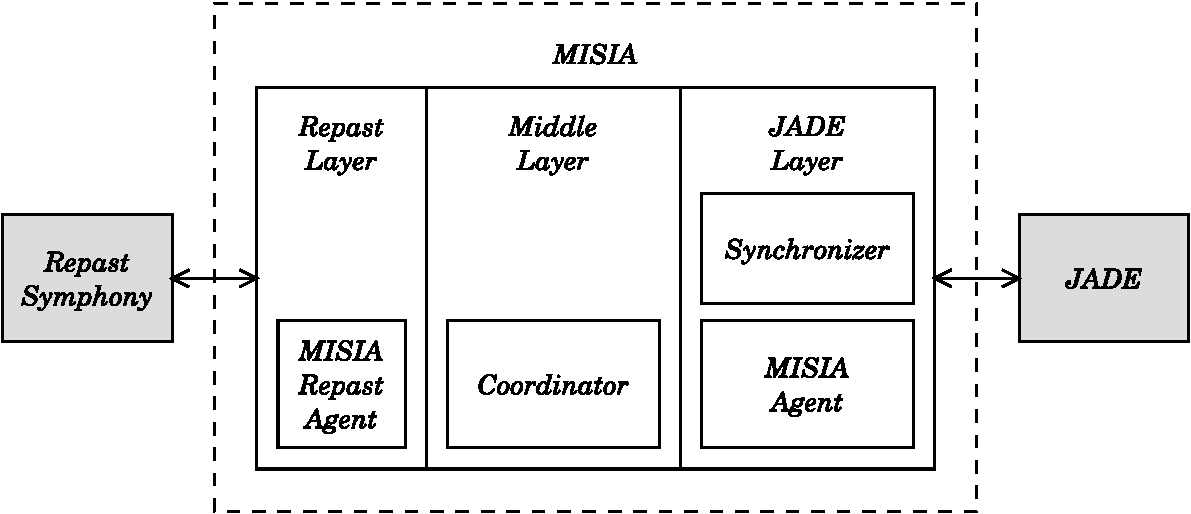
\includegraphics[width=0.75\linewidth]{figures/MISIA.pdf}
	\caption[MISIA's architecture]{High-level representation of MISIA's architecture (adapted from \cite{garcia2011misia})}
	\label{fig:misia}
\end{figure}

One of the challenges identified by the authors when re-implementing the FIPA interaction protocols was synchronizing them with the Repast tick-based simulation model. Given JADE's event-driven architecture, MISIA proposes the use of a coordinator agent that informs the JADE-Agent when a tick has passed. It also proposes its own implementation of the interaction protocols supported by JADE, making them tick-friendly.

\subsection{JRep}
JRep is another platform for integrating JADE and Repast Symphony in the same framework, by means of a middleware. To demonstrate its use, the authors present an example of a smart airport and how it can be simulated using JREP.

JRep's approach is not as complex as MISIA's.
By having the Repast Simphony agent encapsulate a JADE agent representation, synchronization is immediate and is assured without requiring an external coordinator.
The two agent representations take care of synchronizing any state changes.
Figure \ref{fig:jrep} represents the basic structure of JRep.

\begin{figure}[h]
	\centering
	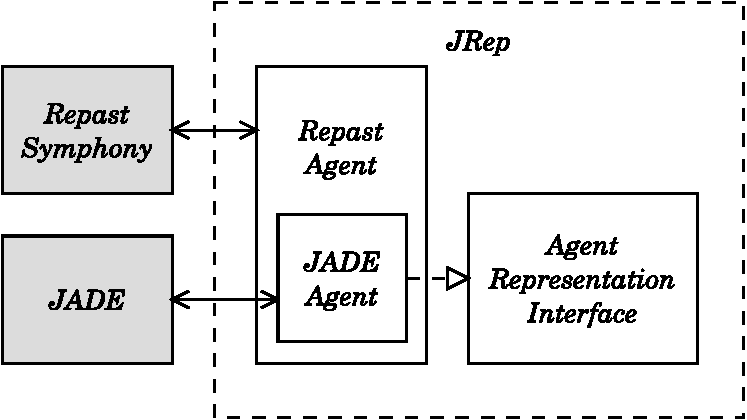
\includegraphics[width=0.5\linewidth]{figures/jrep.pdf}
	\caption[JRep's architecture]{High-level representation of JRep's architecture (adapted from \cite{gormer2011jrep})}
	\label{fig:jrep}
\end{figure}

Each agent takes care of interfacing their respective frameworks. The interaction between agents in JRep is performed using FIPA ACL and the protocol implementations are those provided by the JADE platform. Similarly to MISIA, an Agent Representation Interface is used to introduce the concept of schedule in the JADE agent.

\subsection{PlaSMA}
Unlike the two previous frameworks, the PlaSMA system is based solely on the JADE platform. The distributed simulation is synchronized by entities called ``Controllers'' who communicate with the ``Top Controller'', keeping the pace of the simulation and handling agent lifecycle management as well. Figure \ref{fig:plasma} illustrates this architecture. PlaSMA, unlike MISIA and JRep, is still an active project.

\begin{figure}[h]
	\centering
	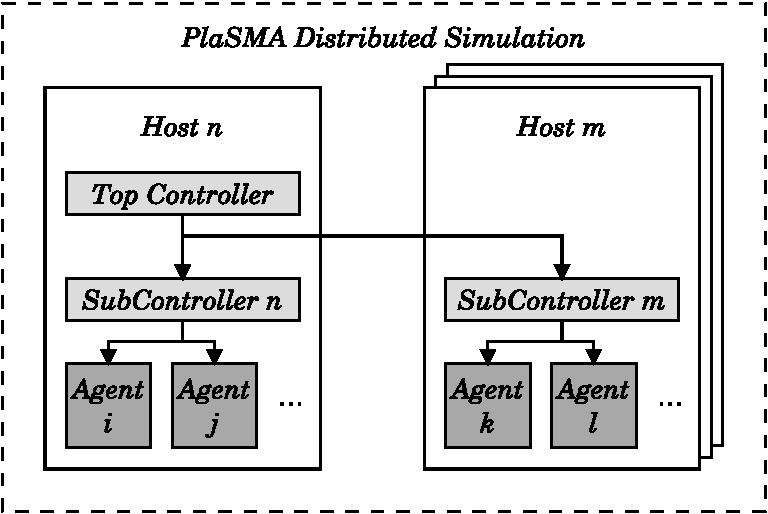
\includegraphics[width=0.5\linewidth]{figures/PlaSMA.pdf}
	\caption[PlaSMA's architecture]{High-level representation of PlaSMA's architecture (adapted from \cite{warden2010towards})}
	\label{fig:plasma}
\end{figure}

JADE is a very rich platform but, for many simulation scenarios, the overhead introduced by it has a significant impact on simulation performance \cite{mengistu2008scalability}.

Even though both MISIA and JRep attempt to integrate the features from both JADE and Repast, as far as Repast simulations are concerned JADE's multi-threaded infrastructure affects their performance very significantly. The main advantage of our approach is, therefore, the possibility of using Repast with JADE features, namely FIPA specifications including interaction protocols, without the need to interface with JADE. 

\section{JADE and Repast}
\label{sec:jade-repast}

To achieve the goals of this thesis, two frameworks were chosen: JADE and Repast. Both are very popular and in widespread use and have been the foundation of the creation of other tools. They are also free and open source and extensively documented.

JADE is a framework for development of FIPA-compliant fully featured MAS. It aims at simplifying the creation of distributed agent applications by seamlessly hiding all complexity regarding its distributed architecture, including the tasks of agent discovery and the handling of messages.

Repast is a toolkit that provides an environment for the creation of MABS using POJO\footnote{Plain Old Java Objects}. It makes it fairly simple to collect agent data and generate displays for it, including charts, grids and others.

\begin{table}[h]
	\caption{Summary of JADE and Repast features.}
	\label{tab:jadevsrep}
	\begin{center}
		\begin{tabular}{l|cc}
		\hline

		\hline
		\textbf{} & \textbf{JADE} & \textbf{Repast} \\ %& \textbf{Cougaar} \\
		\hline
			Communication & FIPA ACL &  Method calls  \\ %& Serialized Object \\
						  &			 &  Shared resources \\
		\hline
			Distribution & Yes & No \\ %& Yes \\
		\hline
			Simulation Tools & No & Yes \\ %& Yes \\
		\hline
			Scalability & Limited & High \\ %& High \\
		\hline
			Ontologies & Yes & No \\ %& Yes\\
		\hline
			Open Source & Yes & Yes \\ %& Yes\\
		\hline
			Agent Execution & Behaviour-based & Schedule-based  \\ %&  \\
							& Multi-threaded & Single-threaded \\ %&  \\
							& Event-driven   & Tick-driven 	   \\ %&  \\
							& Assync		 & Sync 		   \\ %&  \\
		\hline
		\end{tabular}
	\end{center}
\end{table}

In JADE, as table \ref{tab:jadevsrep} illustrates, agents execute in separate threads and while this architecture facilitates the platform's distribution, JADE's agent are heavy in terms of resources. Experiments with JADE show that the platform's scalability is limited in number of agents and that the global system performance drops quickly for large number of agents \cite{mengistu2008scalability} \cite{garcia2011misia}. This further strengthens the idea that using JADE or a JADE-Repast hybrid, as describe in the related work, is not the best course of action is performance is an important issue.

In Repast, agent execution is scheduled manually. An agent class can contain annotations that indicate which methods should be called and when (for instance every tick or every 100 ticks). This approach is very flexible, allowing to schedule any method but more complex structures are non-existent in Repast.

In contrast, JADE agent actions can be executed in their setup and takedown, but most are encapsulated in objects called Behaviours. JADE has many different kinds of behaviours that function in different ways, such as running one single task once or running them cyclically. Other behaviours implement FIPA interaction protocols, which agents can use to interact with other agents.

Agents, as well as their behaviours, go through different states, as Figure \ref{fig:jade_fluxogram} suggests. As each agent in JADE runs in a thread, each one is dedicated solely to the agent's behaviours. These behaviours are executed consecutively until the agents is taken down and each behaviour stops being scheduled when it is ``done'' -- indicated by the return value of the method \texttt{done()}.

\begin{figure}[h]
	\centering
	\includegraphics[width=0.7\linewidth]{figures/jade_fluxogram.pdf}
	\caption[JADE Behaviour execution states]{JADE Behaviour execution states and events (adapted from \cite{bellifemine2007developing})}
	\label{fig:jade_fluxogram}
\end{figure}

%!TEX root = ../thesis.tex
\section{FIPA Specifications in JADE} % (fold)
\label{sec:fipa}

% Intro to FIPA in JADE/API
\apiname{} closely follows JADE's architecture regarding the use of protocols and services specified by FIPA. 
%The architecture of the API described in this paper includes multiple concepts proposed by FIPA: the \gls{DF}, the \gls{MTS}, the \gls{AMS}, the \gls{ACL} Message and the Interaction Protocols. The following is a brief description of these concepts and of how JADE uses and implements them.

%\begin{figure}
%	\centering
%	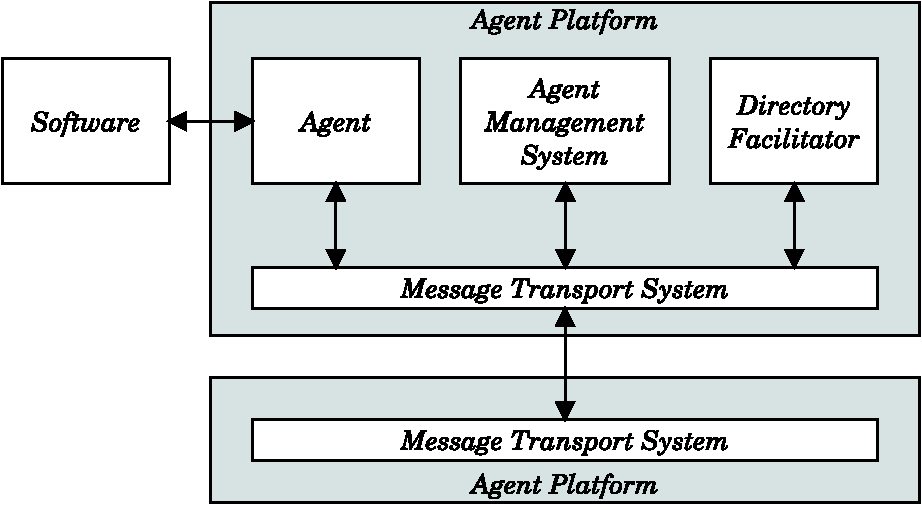
\includegraphics[width=2.5in]{figures/pdf/AMSdiagram.pdf}
%	\caption{
%		Agent Management Reference Model, as specified by FIPA and implemented by JADE. \apiname{} only supports a single Agent Platform.
%	}
%	\label{fig:AMSdiagram}
%\end{figure}

% DF 
The Directory Service (DF) is a component that provides a yellow page service and is part of the FIPA Agent Management Specification. It allows one agent to perform searches about agents rendering specific services. Only agents that are registered in the DF will be indexed and agents can register and deregister themselves at any time.

% DF Agent Description
When searching the DF, agents can use templates that filter the search results. A DF Agent Description represents this template and contains the fields listed in Table \ref{tab:dfAgentDescription}.sim


% MTS
The MTS is a service for transportation of ACL messages between agents. It is responsible for resolving agent addresses, in order to be able to deliver those messages. The MTS may request information from the AMS to perform this address resolution.

% AMS
The AMS is a mandatory component in FIPA-compliant agent platforms. Its purpose is to manage the agent platform, namely the creating and deletion of agents.

% ACL Message
The ACL Message is the envelope that contains the details for communication. The Agent Comunication Language (ACL) stipulates what fields a message should contain. Table \ref{tab:fipaACLMessage} was adapted from the FIPA ACL Message structure specification and contains the list of fields in a message. Not all of them are mandatory. FIPA specifies the \texttt{performative} as the only mandatory field, although the \texttt{sender}, \texttt{receiver} and \texttt{content} are expected to be present.

\begin{table}
	\normalsize
	\caption{FIPA ACL Message Parameters}
	\label{tab:fipaACLMessage}
	\begin{center}
		\fboxsep1pt
		\begin{tabular}{c|c}
		\hline
		\textbf{Parameter} & \textbf{Category of Parameters} \\
		\hline
		\colorbox{Apricot}{\texttt{performative}} & Type of communicative acts \\
		\hline
		\colorbox{Apricot}{\texttt{sender}} & \multirow{3}{*}{Participant in communication} \\
		\cline{1-1}
		\colorbox{Apricot}{\texttt{receiver}} \\
		\cline{1-1}
		\texttt{reply-to}  \\
		\hline
		\colorbox{Apricot}{\texttt{content}} & Content of message \\
		\hline
		\texttt{language} & \multirow{3}{*}{Description of Content} \\
		\cline{1-1}
		\texttt{encoding} \\
		\cline{1-1}
		\colorbox{Apricot}{\texttt{ontology}} \\
		\hline
		\colorbox{Apricot}{\texttt{protocol}} & \multirow{5}{*}{Control of conversation} \\
		\cline{1-1}
		\colorbox{Apricot}{\texttt{conversation-id}} \\
		\cline{1-1}
		\texttt{reply-with} \\
		\cline{1-1}
		\texttt{in-reply-to} \\
		\cline{1-1}
		\colorbox{Apricot}{\texttt{reply-by}} \\
		\hline
		\end{tabular}
	\end{center}
\end{table} 

% Protocols In FIPA
FIPA Interaction Protocols typify communication interactions among agents by specifying two roles: initiator (the agent starting the interaction) and responder (a participant in the interaction). Each protocol defines precisely which messages are sent by each role ad in which sequence.

% Behaviors in JADE
In JADE, every agent activity is programmed through the notion o behaviours. For interaction protocols, typically behaviour-pairs are used for each side of the interaction, and JADE's API supports the most important protocols with built-in initiator and responder behaviours.
% Implementing these protocols.
In order to create an application using these protocols, programmers only need to extend these behaviours and implement the message handlers.
All the complexity regarding the interaction and networking infrastructure is hidden and taken care of by JADE, allowing the programmer to focus on the implementation of agent behaviour.

\subsection{FIPA Interaction Protocols}

To provide a more solid background to the protocols mentioned in this thesis, it's relevant to perform a deeper analysys of them. The two protocols currently supported in the API, as will be explained further ahead in Chapter \ref{chap:solution}, are the FIPA Request, FIPA Query and the FIPA Contract Net. JADE supports a few other protocols, namely FIPA Propose, Iterated FIPA Request and Query and FIPA Subscribe.

\begin{table}
	\normalsize
	\caption{Interaction protocols supported in JADE}
	\label{tab:fipa_protos}
	\begin{center}
		\fboxsep1pt
		\begin{tabular}{c|c|c}
		\hline
		\textbf{Protocol(s)} & \textbf{Initiator class} & \textbf{Initiator class} \\
		\hline
		FIPA request 	& \multirow{2}{*}{AchieveREInitiator} & \multirow{2}{*}{AchieveREResponder}\\
		FIPA Query 		& \\
		\hline
		\multirow{2}{*}{FIPA Contract Net} & \multirow{2}{*}{ContractNetInitiator} & ContractNetResponder \\
		 &  & SSContractNetResponder \\
		\hline
		\end{tabular}
	\end{center}
\end{table}


In JADE, the AchieveRE protocol encompases the multiple ``request-like'' behaviours such as FIPA-Request. It is a simple protocol with three moments of interaction, as Figure \ref{fig:FIPA_request_proto} shows: a request, a response of acceptance or refusal and a facultative result notification. JADE allows the use of other interaction protocols with the AchieveRE: FIPA-query, FIPA-Request-When, FIPA-recruiting and FIPA-brokering. Interaction using this protocol can be 1:1 or 1:N.

The Contract Net protocol starts with a Call for Proposals (CFP) sent to one or more agents, which can reply with a proposal or with a refusal to propose. The initiator can then accept or reject the proposals. As in FIPA-Request, the final result notification is facultative. The ContractNetResponder class from JADE resets itself after terminating the protocol and stays waiting for new CFPs. JADE provides an alternative responder class called SSContractNetResponder that terminates after a single session (SS stands for single session).

\begin{figure}[ht]
	\centering
    \begin{subfigure}[b]{0.44\textwidth}
		\centering
		\includegraphics[height=4in]{figures/FIPA_request_proto.pdf}
		\caption[FIPA-Request protocol]{FIPA-Request protocol}
		\label{fig:FIPA_request_proto}
    \end{subfigure}%
    \begin{subfigure}[b]{0.54\textwidth}
		\centering
		\includegraphics[height=4in]{figures/FIPA_contnet_proto.pdf}
		\caption[FIPA-Contract-Net protocol]{FIPA-Contract-Net protocol}
		\label{fig:FIPA_contnet_proto}
    \end{subfigure}
    \caption[]{Sequence diagrams for the protocols Contract Net and Request. \\Figures are from the FIPA specifications website \footnote{http://fipa.org/})}
    \label{fig:FIPA_Protocols}
\end{figure}


\section{Summary}
Although the specific problem of reimplementing JADE features in Repast using a pure Java approach has not been approached before in the available literature, it is clear that some related work is useful in the definition of the solution proposed in this thesis. 

JREP and MISIA show that interoperability between the two frameworks is possible and they helped understand the limitations of each framework. They both attempted to complement Repast's lack of communication protocols by creating an interface with JADE's implementation of FIPA interaction protocols. The usefulness of these works is limited, though, since the source code is not readily available and neither project is still being developed and supported.

Other works related to the integration of features from Repast and JADE are available and these were selected as the most relevant. While the goal of this thesis is not to use both frameworks simultaneously, these works give a valuable insight into the shortcomings of both frameworks as well as providing some interesting comparisons between their features. Open source projects exist that contemplate the use of FIPA ACL as a library, but none was found to be actively maintained or properly documented. Therefore, this thesis contemplates the creation of a Java API that brings JADE-like features to simulation tools, including FIPA standards.
%!TEX root = ../thesis.tex
\chapter{Closening MAS Simulation and Development through a JADE-based API}
\label{chap:solution}

The modelling of MAS can be accomplished through the use of a wide range of available platforms, as explained before. In certain cases, in order to benefit from different features, modelling the same system in multiple development environments may be necessary.

As explained in Introduction, the two mains goals of this thesis are the creation of an adapter to provide abstraction from MABS frameworks, allowing the creation of JADE-based simulations, and the creating of a mechanism that uses this adapter to convert MABS into MAS. To accomplish these goals, an integrated system was designed, which comprises two main components :

\begin{enumerate}
  \item The \textbf{Simple API for JADE-based Simulations (\apiname{})}, which provides a set of features present in JADE; those features were reimplemented from scratch in an attempt to simplify their internal complexity, preserving JADE-like external execution;
  \item The \textbf{\pluginname (\plugin)} in the form of an Eclipse plug-in that is capable of mapping JADE and \apiname{} features and convert applications developed using one into applications based on the other, automatically. The plugin has no Repast or JADE dependencies in the code, buts contains a dictionary file that is specific to JADE and Repast.
\end{enumerate}

This chapter makes a high level overview of both components and how they work together. After an overview in the next section, Section \ref{sec:solution-fipa} explains how FIPA standards for agent interaction and management are implemented in \apiname{}. Section \ref{sec:solution-scenarios} contains a description of the expected scenarios where this system could be used.

\section{Overview}
\label{sec:solution-overview}
%In this section, explain the integrated solution of \apiname{} + plug-in, how they work, what they use in terms of dependencies, etc.

\apiname{} is an API meant to be used with simulation frameworks to enable JADE-based features in them, including agent interaction protocols and agent management services. The API also uses JADE's concept of behaviours which encapsulate most of agents' actions.

\apiname{} was initially created to be used with Repast Simphony. However, it was developed in a way that allows its integration with other simulation tools. The interface between Repast and \apiname{} is made in a single point, the Scheduler, which is a Repast-specific structure. If developers desire to add support for other simulation frameworks, different implementations of the scheduler can be created.

Another important aspect kept in mind when developing \apiname{} was the importance of keeping a close semblance to JADE's own API not only to make the code  conversion more straightforward, but to allow proficient JADE developers to create \apiname{}-based simulations using a familiar JADE-based API. \plugin was developed as an Eclipse plugin. It provides programmers with two possible actions: convert code from JADE to \apiname{} and in the opposite direction.

\apiname{} does not yet implement all JADE features. For the purposes of this thesis, a set of the most common features were selected which allows for the simulation of scenarios with some complexity, including negotiation between agents and the creation of custom behaviours. Features in JADE applications which are not available in \apiname{} will typically be shown as errors when converted; \plugin simply ignores them and they should be re-implemented manually as necessary. Chapter \ref{chap:validation} shows examples of scenarios created with \apiname{} and JADE that were successfully converted while preserving functionality.

Figure \ref{fig:related-repacl} tries to compare \apiname{} with JRep and MISIA, described in Chapter \ref{chap:background}. The API's general structure is simpler; it does not intend to maintain an active connection to a JADE platform, eliminating the need for synchronization. Instead, our goal is to replicate in our API the main features of JADE, allowing for a straightforward and dependency free feature mapping between \apiname{} and JADE.

\begin{figure}
	\centering
	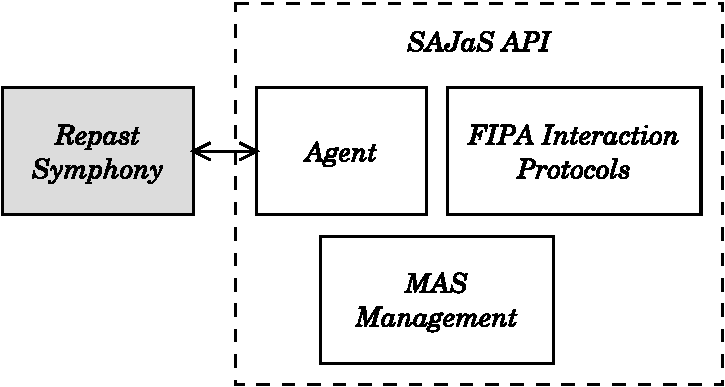
\includegraphics[width=0.5\linewidth]{figures/repacl.pdf}
	\caption{Basic structure of \apiname{}}
	\label{fig:related-repacl}
\end{figure}

\section{FIPA Specifications}
\label{sec:solution-fipa}

Part of the rationale for the creation of \apiname{} was to enable agent interaction standards in otherwise standard-less simulation frameworks, namely Repast, the one featured in this thesis. This section explains the FIPA standards for agent interaction and management implemented in \apiname{}.

As mentioned before, \apiname{} follows JADE architecture very closely, including how FIPA standards are implemented. The implemented features can be divided in the following categories:

\begin{enumerate}
  \item \textbf{Agent Management}, which includes the directory facilitator (DF) service, the structures used by it and the Agent Management Service (AMS),
  \item \textbf{Messaging}, including the ACL Message, the Message Template and the Message Transport Service (MTS), and
  \item \textbf{Interaction Protocols} that allow agents to exchange ACL Messages in a standardized manner.
\end{enumerate}

\subsection{Agent Management}
The AMS functions as a directory of all agents in a MAS and every agent is automatically registered in the AMS upon its initialization. BY the time they are registered, agents are also assigned an Agent Identifier (AID) used throughout the application. Only the AMS and the agent itself know who the AID belongs to.

The DF is a facultative directory where agents can register themselves as service providers. The DF Agent Description is a structure used to describe one agent when it registers itself in the DF or to describe a group of agents when performing a search. The DF Agent Description can contain one or more Service Descriptions. The fields of these structures are listed in Table \ref{tab:dfAgentDescription}.

\begin{table}
	\normalsize
	\caption[The DF Agent Descriptions and the Service Description]{Information contained in the DF Agent Descriptions and Service Description structures.
	M: Mandatory field. S: Mandatory when agent registers.}
	\label{tab:dfAgentDescription}
	\begin{center}
		\begin{tabular}{c|c}
		\hline
		\textbf{DFAgentDescription} & \textbf{ServiceDescription} \\
		\hline
		name \textsuperscript{S} : AID & service name \textsuperscript{M} : String \\
		\hline
		services : ServiceDescriptions & type \textsuperscript{M} : String \\
		\hline
		\multicolumn{2}{c}{protocols : Strings} \\
		\hline
		\multicolumn{2}{c}{ontologies : Strings} \\
		\hline
		\multicolumn{2}{c}{languages : Strings} \\
		\hline
		\end{tabular}
	\end{center}
\end{table} 

\subsection{Messaging}
The implementation of the ACL Message is essentially identical to JADE's. \apiname{} also implements the Message Template, which is used to filter incoming messages. A series of template factories exist in the API that allow one to create message templates. 

\subsection{Interaction Protocols}
% The interaction protocols in the api
JADE has the support for many interaction protocols. The most common ones were selected to be included in \apiname{}.
% The specific protocols
The implemented protocols were the ``request-like'' Achieve Rational Effect (AchieveRE) protocol, the Contract Net protocol and the Single Session Contract Net - including the Responder Dispatcher behaviour, which uses it.

The AchieveRE encompasses multiple FIPA protocols, namely Request, Query, Request-When, Recruiting and Brokering protocols, as defined in JADE's documentation.

\section{Usage Scenarios}
\label{sec:solution-scenarios}
%In this section, show how the whole setup is used with detailed use cases
This section is meant to describe both the scenarios where this system is expected to be useful, as well as the actual possible use cases. Figure \ref{fig:prototypeFlow} illustrates these scenarios.

\begin{figure}
	\centering
	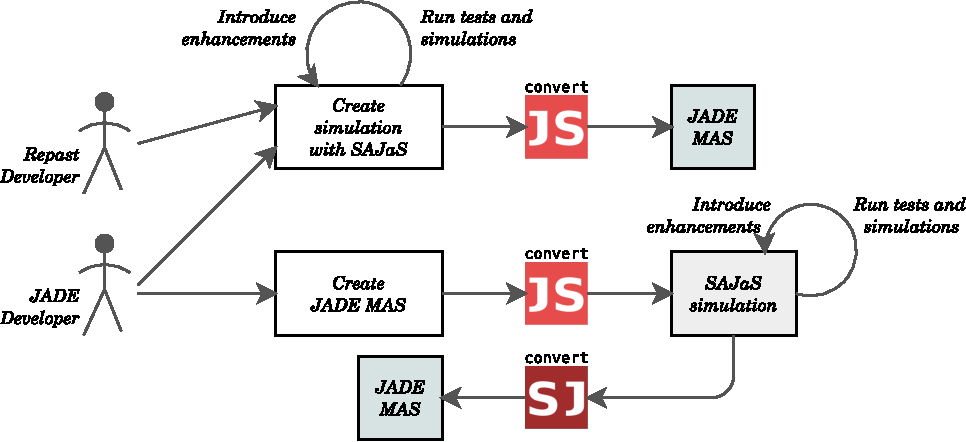
\includegraphics[width=\linewidth]{figures/prototypeFlow.pdf}
	\caption{
		Possible work flows for \apiname{} users. ``SJ'' and ``JS'' represent conversion from SAJaS to JADE and the reverse, respectively.
	}
	\label{fig:prototypeFlow}
\end{figure}

One possible scenario is when a JADE developer created a JADE MAS and desires to perform some tests and simulations in a local and controlled environment. The developer can use this tool to convert the MAS into a MABS. Eventually, the application can be converted back if changes were made while in the simulation format.

A second possible scenario could be that of a developer that intends to create a MABS with the goal of later creating a MAS out of it. This could be a Repast developer who desires to create more complex agent simulations or a JADE developer that wants to create Repast simulations using familiar JADE-like tools.

A third scenario is when a developer simply wants to create a complex agent-based, FIPA-compliant simulation. In this case, there is no need for a code conversion tool, but \apiname{} can be used as a standalone library.

\section{Summary}

In this chapter, SAJaS was presented as part of the solution to accomplish this thesis' goal of bringing MAS development and simulation. This high level description of the API comprised an overview of its main features. In the next chapter, an analysis of SAJaS' implementation is provided, allowing for a deeper understanding of how it works internally and how it differs from JADE -- together with a justification of why their implementation is no identical.
%!TEX root = ../thesis.tex
\chapter{Software Architecture}
\label{chap:architecture}
%!TEX root = ../thesis.tex
\chapter{Validation}
\label{chap:validation}

The main goal of this thesis was to develop a solution for bridging the gap between the simulation and MAS domains that, while maintaining a familiar JADE-like environment, would offer significant performance improvements to MABS development. To validate this approach and the developed tools, a set of experiments were designed, in an attempt to cover and test all the available features.

The first example consists in a simple contract net between one buyer and multiple sellers. In the second example, multiple contract nets run concurrently and some of the buyers include available computational trust about sellers. The third example is a board game called Risk developed prior to this thesis. The goal of this last example was to test SAJaS in a ``real'' example of an already developed MAS, one that had not been developed specifically for this thesis. All tests were performed in a laptop using an Intel i7 CPU (8 logical cores) at 2.20 GHz and 8GB of RAM.

%!TEX root = ../thesis.tex
\section{Simple Contract Net}

In this scenario, one agent sends a call for proposals (CFP) to multiple agents which then reply with their individual proposals. This simple scenario was created to test the core of SAJaS and the plugin. The goal was not only to create a working simulation model based on SAJaS, but also to demonstrate that the execution of a simulation in SAJaS and the equivalent JADE application generated from it are identical and that performance in SAJaS is higher. For that purpose, this scenario was developed as a simulation in SAJaS and Repast and then converted to a JADE MAS.

\subsection{Experimental Setup}

The diagram in Figure \ref{fig:CNetExample} illustrates the contract net created for this test. An agent (the buyer) intends to purchase a certain quantity of three kinds of goods: rice, flour and oats. Besides the quantities of each product it needs, the buyer also stipulates a maximum price for the whole deal. The buyer will issue a call for proposals (CFP) containing a request for supplies to all agents that announce themselves as suppliers in the DF.

Supplier agents have a maximum supply capacity and a price for each product. After receiving a CFP, the supplier replies with a PROPOSAL containing a price for each product if the demanded supply is within the seller's capacity. Otherwise, a REFUSE message will be sent to the buyer.
Finally, the buyer agent compares all valid proposals, chooses the cheapest offer for each of the three products and replies with an ACCEPT PROPOSAL to the best offers, and REJECT PROPOSAL to all others.

\begin{figure}
	\centering
	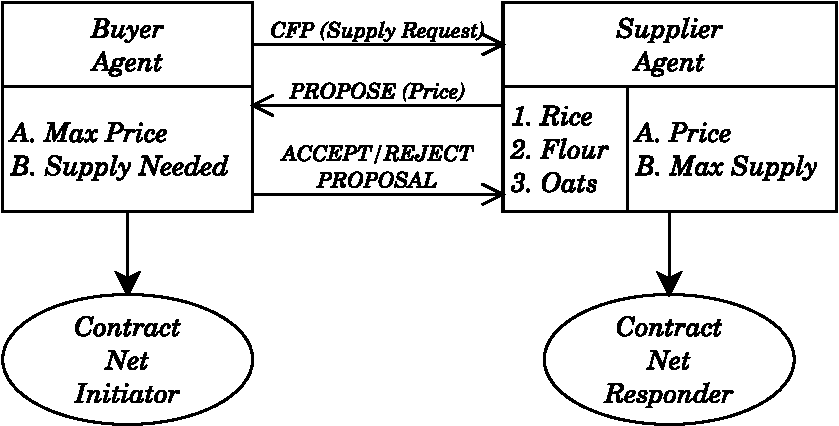
\includegraphics[width=0.60\linewidth]{figures/CNetExample.pdf}
	\caption{Representation of the contract net scenario.}
	\label{fig:CNetExample}
\end{figure}

To ensure the proper comparison of results, a fixed data set with values for prices and demand was used in both frameworks. This experiment focused on two simple metrics to evaluate the result: time and outcome. 

Multiple executions were performed with varying numbers of suppliers (as sugested by Figure \ref{fig:performance}); for each case, the simulation was executed 10 times. The execution time was measured from the begining of the protocol, until all suppliers were notified.

In JADE, the simulation was tested in two different setups: first, with all agents running in a single container; second, with the supplier agents in one container and the buyer in a separate one (but in the same host). In this configuration, all communication between agents happens across containers. The second validation metric was the actual result of the protocol, i.e who were the supplier agents chosen by the buyer and their price proposals.

\subsection{Results}

After 10 executions, the average performance of the experiment was calculated for each number of agents and is represented in Figure \ref{fig:performance}. The performance of the simulation based on SAJaS was significantly better, excelling when the number of agents is high. JADE was able to perform better when using two distinct containers.
%JADE's performance drops very significantly when there is a high communication-to-computation ratio in the application\cite{mengistu2008scalability}.

Regarding the outcome of the protocol, the same values were obtained in both implementations for each number of agents, confirming that the execution is identical in both implementations.

\begin{figure}
	\centering
	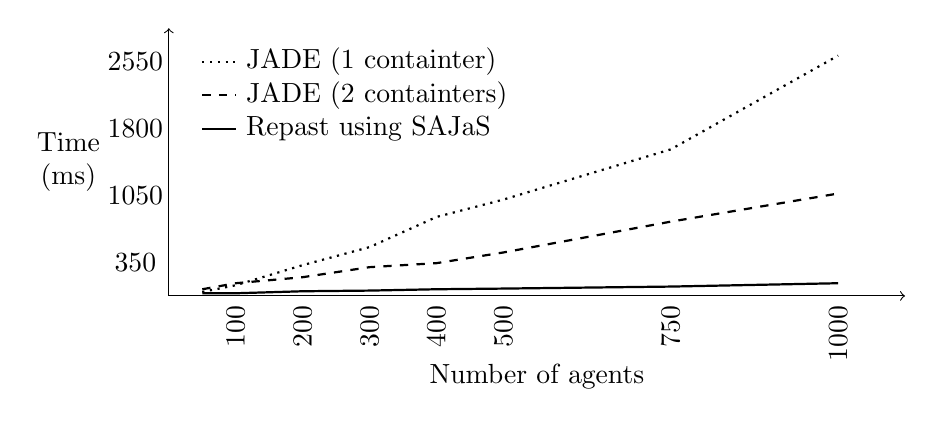
\begin{tikzpicture}[scale=0.85]

		% horizontal axis
		\draw[->] (0,0) -- (11,0);
		\draw (5.5,-1.2) node[align=center] {Number of agents}; %label

		
		% labels
		\draw	%(0.5,0) node[rotate=90, anchor=east] {50}
				(1.0,0) node[rotate=90, anchor=east] {100}
				(2.0,0) node[rotate=90, anchor=east] {200}
				(3.0,0) node[rotate=90, anchor=east] {300}
				(4.0,0) node[rotate=90, anchor=east] {400}
				(5.0,0) node[rotate=90, anchor=east] {500}
				(7.5,0) node[rotate=90, anchor=east] {750}
				(10.,0) node[rotate=90, anchor=east] {1000};

		\draw	(-0.5,0.5) node[anchor=center] {350}
				(-0.5,1.5) node[anchor=center] {1050}
				(-0.5,2.5) node[anchor=center] {1800}
				(-0.5,3.5) node[anchor=center] {2550};
		% vertical axis
		\draw[->] (0,0) -- (0,4);
		\draw (-1.5,2) node[align=center] {Time\\(ms)}; %label
		%\draw (-1.5,1.6) node[align=center] {(ms)}; %label

		%% Data %%
		% JADE 2 containers
		\draw[thick,dashed] (0.5,3.0) --
			(1,3.0) node[anchor=west, pos=1.0] {JADE (2 containters)}; %subtitle
		\draw[thick,dashed] (0.5, 0.10) --
					(1.0, 0.19) --
					(2.0, 0.28) --
					(3.0, 0.43) --
					(4.0, 0.49) --
					(5.0, 0.65) --
					(7.5, 1.11) --
					(10., 1.53);
		% JADE 1 containers
		\draw[thick,dotted] (0.5,3.5) --
			(1,3.5) node[anchor=west, pos=1.0] {JADE (1 containter)}; %subtitle
		\draw[thick,dotted] (0.5, 0.06) --
					(1.0, 0.16) --
					(2.0, 0.46) --
					(3.0, 0.73) --
					(4.0, 1.18) --
					(5.0, 1.44) --
					(7.5, 2.19) --
					(10., 3.59);
		% Repast
		\draw[thick] (0.5,2.5) --
			(1,2.5) node[anchor=west, pos=1.0] {Repast using \apiname{}}; %subtitle
		\draw[thick] (0.5, 0.04) --
					(1.0, 0.04) --
					(2.0, 0.07) --
					(3.0, 0.08) --
					(4.0, 0.10) --
					(5.0, 0.11) --
					(7.5, 0.14) --
					(10., 0.19);


	\end{tikzpicture}
	\caption[Execution performance in a simple contract net]
	{Average execution time of each framework in the different experiments.}
	\label{fig:performance}
\end{figure}

%!TEX root = ../thesis.tex
\section{Multiple Contract Net using Trust}

This scenario is similar to the previous one, but attempts to perform a better coverage of the features present in SAJaS, namely the use of the AchieveRE Protocol and the Responder Dispatcher which allows for multiple contract nets to be handled without deadlocks occuring. However. rather than comparing the exact value obtained from the simulation as in the previous scenario, the goal is to compare the overall behaviour of all agents.

\subsection{Experimental Setup}
This simulation is composed by multiple buyers and multiple sellers running simultaneously. After the sellers register themselves in the DF, each buyer will perform a search for sellers of the particular good it needs to purchase. Then, the buyer sends this list of agents to the CTAgent (CT standing for computational trust). The CTAgent will calculate a trust value for each seller based on its past contracts with buyers and return the top 5 sellers.

With this information, the buyer sends a CFP only to the 5 top agents and accept the best proposal from them. Some sellers will occasionally violate the contract after acceptance. The buyer will then inform the CTAgent if the contract was fulfilled or violated. The compilation of this composes the trust of the seller.

Some buyers are programmed to ignore trust and rely solely on the proposal. The idea is that informed buyers eventually avoid contacting sellers programmed to violate contracts more often. The goal of this experiment is to model this scenario in SAJaS, convert it to JADE and verify that the obtained results are very similar.

After one contract is concluded, Buyers start a new one, performing a new DF search for the next product they want to buy, request information from the CTAgent and issuing a new CFP.

\subsection{Results}

The experiment was executed 5 times in JADE and 5 times in SAJaS. The scenario is composed of 20 buyers using computational trust, 20 not using trust and 80 sellers. A total of 2000 contracts were recorded to create the following charts in Figures \ref{fig:enterprise_JADE} and \ref{fig:enterprise_SAJaS}. As shown, buyers who made use of computational trust had more successful contracts. The fluctuations early in the simulation are due to the initial lack of trust information.

As expected and as shown in the charts, the same outcome was observed both in JADE and SAJaS. With this experiment, it was possible to test the Request protocol - when requesting computational trust, the Contract Net - when purchasing goods, the Responder Dispatcher - to handle CFPs from multiple buyers concurrently, the messaging system and the DF service.

In terms of performance, the outcome of this experiment, as ilustrated by the chart in Figure \ref{fig:enterprise_times}, may not seem as impressive when compared with the first experience. However, the algorithm employed to calculate trust is very time consuming. In a setup without the use of trust by any of the buyers, the performance difference between JADE and SAJaS is comparable to the first scenario.

\begin{figure}[ht]
	\centering
	\begin{subfigure}[b]{\textwidth}
		\centering
		\begin{tikzpicture}[scale=0.85]

			% horizontal axis
			\draw[->] (0,0) -- (11,0);
			\draw (5.5,-1.2) node[align=center] {Number of Contracts}; %label

			% labels
			\draw	(0  ,0) node[anchor=north] {0}
					(2.5,0) node[anchor=north] {500}
					(5  ,0) node[anchor=north] {1000}
					(7.5,0) node[anchor=north] {1500}
					(10 ,0) node[anchor=north] {2000};
			
			
			% vertical axis
			\draw[->] (0,0) -- (0,5);
			\draw (-1.1,2.5) node[rotate=90, anchor=south, align=center]
				{\% of Fullfielment}; %label
			\draw	(0, 1) node[anchor=east] {0.25}
					(0, 2) node[anchor=east] {0.50}
					(0, 3) node[anchor=east] {0.75}
					(0, 4) node[anchor=east] {1.00};
			
			

			%% Data %%

			%subtitles
			\draw[thick] (0.5,3.5) --
				(1,3.5) node[anchor=west, pos=1.0] {Using trust and proposal};
			\draw[thick, dotted]
				(0.5,4.5) --
				(1,4.5) node[anchor=west, pos=1.0] {Using only the proposal}; 

			%lines
			\input{chapters/charts/enterprise_values_jade}


		\end{tikzpicture}
		\caption{In SAJaS}
		\label{fig:enterprise_JADE}
	\end{subfigure}
	\bigskip\\
	\begin{subfigure}[b]{\textwidth}
		\centering
		\begin{tikzpicture}[scale=0.85]

			% horizontal axis
			\draw[->] (0,0) -- (11,0);
			\draw (5.5,-1.2) node[align=center] {Number of Contracts}; %label

			% labels
			\draw	(0  ,0) node[anchor=north] {0}
					(2.5,0) node[anchor=north] {500}
					(5  ,0) node[anchor=north] {1000}
					(7.5,0) node[anchor=north] {1500}
					(10 ,0) node[anchor=north] {2000};
			
			
			% vertical axis
			\draw[->] (0,0) -- (0,5);
			\draw (-1.1,2.5) node[rotate=90, anchor=south, align=center]
				{\% of Fullfielment}; %label
			\draw	(0, 1) node[anchor=east] {0.25}
					(0, 2) node[anchor=east] {0.50}
					(0, 3) node[anchor=east] {0.75}
					(0, 4) node[anchor=east] {1.00};

			%% Data %%

			%subtitles
			\draw[thick] (0.5,3.5) --
				(1,3.5) node[anchor=west, pos=1.0] {Using trust and proposal};
			\draw[thick, dotted] 
				(0.5,4.5) --
				(1,4.5) node[anchor=west, pos=1.0] {Using only the proposal}; 
			
			%lines
			\input{chapters/charts/enterprise_values_sajas}


		\end{tikzpicture}
		\caption{In JADE}
		\label{fig:enterprise_SAJaS}
	\end{subfigure}
	\caption[Multiple Contract Net scenario results in JADE]
	{Average result of 5 executions of the Multiple Contract Net scenario during 2000 contracts}
\end{figure}

\begin{figure}
	\centering
	\begin{tikzpicture}[scale=0.85]

		% horizontal axis
		\draw[->] (0,0) -- (11,0);
		\draw (5.5,-1.2) node[align=center] {Time/s}; %label

		% labels
		\draw	(1.4,0) node[anchor=north] {2}
				(2.8,0) node[anchor=north] {4}
				(4.2,0) node[anchor=north] {6}
				(5.6,0) node[anchor=north] {8}
				(7.1,0) node[anchor=north] {10}
				(8.5,0) node[anchor=north] {12}
				(9.9,0) node[anchor=north] {14};
		
		
		% vertical axis
		\draw[->] (0,0) -- (0,5);
		\draw (-1.1,2.5) node[rotate=90, anchor=south, align=center]
			{Number of Contracts}; %label
		\draw	(0, 0) node[anchor=north] {0}
				(0, 1) node[anchor=east] {500}
				(0, 2) node[anchor=east] {1000}
				(0, 3) node[anchor=east] {1500}
				(0, 4) node[anchor=east] {2000};
		
		

		%% Data 
		%subtitle
		\draw[thick] (0.5,3.5) --
			(1,3.5) node[anchor=west, pos=1.0] {SAJaS};
		%line
		\input{chapters/charts/enterprise_times}

		\draw[thick, dotted]%subtitle
			(0.5,4.5) --
			(1,4.5) node[anchor=west, pos=1.0] {JADE}; 


	\end{tikzpicture}
	\caption[Multiple Contract Net scenario results in Repast]
	{Number of contracts executed in JADE and SAJaS. Final number of contracts is 2000 for both frameworks.}
	\label{fig:enterprise_times}
\end{figure}

\input{chapters/validation:risk}


\section{Summary}

These three experiments were designed to validate the results of this thesis.Technically, the scenarios described in this chapter covered all currently available features in SAJaS. The Achieve RE protocol was used in the Enterprise scenario to communicate with the CT Agent and it was widely used in Risk for all communications. The Contract Net protocol was covered in the first two experiments. The Enterprise scenario also allowed multiple concurrent contracts to take place by using the Responder Dispatcher.

All scenarios made use of the DF service, the AMS, the MTS and of containers like the ACL Message, the Message Template, the DFAgentDescription and the Service Description. The creation of custom Simple Behaviours and Finite State Machine (FSM) Behaviours was covered by Risk. It was possible to demonstrate that bringing JADE and Repast together is not only feasible using the developed tools, but also provides increased performance when compared with JADE MAS.



%!TEX root = ../thesis.tex
\chapter{Future Work}
\label{chap:futurework}


%!TEX root = ../thesis.tex
\chapter{Conclusions}
\label{chap:conclusions}

MAS are used in many different domains and research based on simulation has seen an increase in the use of agent-based approaches in their development. As a result, many frameworks for the development of MABS have been created. With a review of the available literature, it is possible to conclude that there is interest in bridging the domains of MAS and MABS. While MABS are typically not used in production, MAS are usually not the most appropriate to perform tests and simulations, more so when large number of agents are in use.

Some works were studied whose motivation was to bridge these domains. MISIA, JRep and PlaSMA proposed approaches that extended the MAS development framework JADE with simulation development features. This thesis proposed an alternative approach in which JADE-based features were included in the MAS framework Repast without relying in JADE libraries -- those features were re-implemented for this purpose.

\section{Main Contributions}
To bridge the gap between MAS development and simulation, the Simple API for JADE-based Simulations (\apiname) was created. JADE developers are able to create Repast-based simulations using familiar JADE features. The \pluginname (\plugin) was also developed to enable the conversion of simulations created with \apiname into JADE MAS.

The main issues detected during the development of \apiname were related to to the different nature of the execution of Repast and JADE. JADE's agents run in multiple threads and global agent synchronization does not exist. Agent interaction happens asynchronously. The kind of simulation frameworks targeted by this API, like Repast, relies on synchronized events that occur consecutively in ``ticks''. By using ACLMessages in Repast and a messaging system that relies on messages being kept in a mail queue, asynchronous agent interaction is possible despite Repast synchronism. Messages are processed when the simulation grants execution the the agent who owns them.

Negotiation scenarios were created to validate both \apiname and \plugin. The goals were to demonstrate that it was possible to create agent-based scenarios with some complexity using \apiname's implemented features and that after its conversion using \plugin was not only feasible, but the resulted MAS displayed identical behaviour when executed. Furthermore, the \apiname version is significantly faster. The two negotiation scenarios showed that a Repast simulation based on \apiname was many times faster than its JADE equivalent.

%!TEX root = ../thesis.tex
\chapter{Future Work}
\label{chap:futurework}



%% comment next 2 commands if numbered appendices are not used
% \appendix
% \chapter{Loren Ipsum} \label{ap1:loren}

Depois das conclusões e antes das referências bibliográficas,
apresenta-se neste anexo numerado o texto usado para preencher a
dissertação.

\section{O que é o \emph{Loren Ipsum}?}

\emph{\textbf{Lorem Ipsum}} is simply dummy text of the printing and
typesetting industry. Lorem Ipsum has been the industry's standard
dummy text ever since the 1500s, when an unknown printer took a galley
of type and scrambled it to make a type specimen book. It has survived
not only five centuries, but also the leap into electronic
typesetting, remaining essentially unchanged. It was popularised in
the 1960s with the release of Letraset sheets containing Lorem Ipsum
passages, and more recently with desktop publishing software like
Aldus PageMaker including versions of Lorem Ipsum~\citep{kn:Lip08}. 

\section{De onde Vem o Loren?}

Contrary to popular belief, Lorem Ipsum is not simply random text. It
has roots in a piece of classical Latin literature from 45 BC, making
it over 2000 years old. Richard McClintock, a Latin professor at
Hampden-Sydney College in Virginia, looked up one of the more obscure
Latin words, consectetur, from a Lorem Ipsum passage, and going
through the cites of the word in classical literature, discovered the
undoubtable source. Lorem Ipsum comes from sections 1.10.32 and
1.10.33 of ``de Finibus Bonorum et Malorum'' (The Extremes of Good and
Evil) by Cicero, written in 45 BC. This book is a treatise on the
theory of ethics, very popular during the Renaissance. The first line
of Lorem Ipsum, ``Lorem ipsum dolor sit amet\ldots'', comes from a line in
section 1.10.32.

The standard chunk of Lorem Ipsum used since the 1500s is reproduced
below for those interested. Sections 1.10.32 and 1.10.33 from ``de
Finibus Bonorum et Malorum'' by Cicero are also reproduced in their
exact original form, accompanied by English versions from the 1914
translation by H. Rackham.

\section{Porque se usa o Loren?}

It is a long established fact that a reader will be distracted by the
readable content of a page when looking at its layout. The point of
using Lorem Ipsum is that it has a more-or-less normal distribution of
letters, as opposed to using ``Content here, content here'', making it
look like readable English. Many desktop publishing packages and web
page editors now use Lorem Ipsum as their default model text, and a
search for ``lorem ipsum'' will uncover many web sites still in their
infancy. Various versions have evolved over the years, sometimes by
accident, sometimes on purpose (injected humour and the like). 

\section{Onde se Podem Encontrar Exemplos?}

There are many variations of passages of Lorem Ipsum available, but
the majority have suffered alteration in some form, by injected
humour, or randomised words which don't look even slightly
believable. If you are going to use a passage of Lorem Ipsum, you need
to be sure there isn't anything embarrassing hidden in the middle of
text. All the Lorem Ipsum generators on the Internet tend to repeat
predefined chunks as necessary, making this the first true generator
on the Internet. It uses a dictionary of over 200 Latin words,
combined with a handful of model sentence structures, to generate
Lorem Ipsum which looks reasonable. The generated Lorem Ipsum is
therefore always free from repetition, injected humour, or
non-characteristic words etc. 


%%----------------------------------------
%% Final materials
%%----------------------------------------

%% Bibliography
%% Comment the next command if BibTeX file not used
%% bibliography is in ``myrefs.bib''
%\bibliographystyle{chicago}
%\bibliographystyle{plainnat}
\PrintBib{myrefs}
\bibliography{myrefs}

%% Index
%% Uncomment next command if index is required
%% don't forget to run ``makeindex pdis-en'' command
%\PrintIndex

\end{document}
